\section{The effect of switching types}
\label{section:switch}
Segregation is a phenomenon taking many different forms. Rather than  limiting the scope to racial segregation, we decided to broaden our view. 
For example, one might delve into the segregation in studies with respect to friendship. 
In this case, for any person \(k\). The neighbours of \(k\) represent the \(k\)'s friends or the persons with whom \(k\) spends most of his time.
In this case, \(k\)'s type, can represent either the classes he is currently taking, or the kind of sports person \(k\) is doing, or more likely, \(k\)'s political beliefs.
In any of these cases, the type of \(k\) is not necessarily set indefinitely.
In these cases, the type of \(k\) might switch, depending on the types of his friends. THis is a sociological process known as conformation and plays a major role in the everyday behaviour of people.\\

This gives rise to a new modification of the model.
For any person \(k\), before moving to a new location, \(k\) has a catagorical probability with to switch to a different type, where 
\[\mathbb{P}(\text{NewType}(k)=t) = \begin{cases} 
 \frac{\#\text{Neighbours of type }t}{\text{Total number of neighbours}}	&\mbox{if } \text{total number of neighbours}>0 \\ 
\mathbbm{1}_{\{t=\text{Type}(k)\}}   &\mbox{if } \text{total number of neighbours}=0
\end{cases}\]
Note that this is well defined, since for total number of neighbours \(> 0\), we have \( \mathbb{P}(\text{NewType}(k)=t) \geq 0\) and \(\sum_{i=0}^{\text{types}}\mathbb{P}(\text{NewType}(k)=t)=1\). An example of how this may effect the equilibrium, is illustrated below:

\begin{figure}[H]
	\centering
    \begin{subfigure}{0.45\textwidth}
        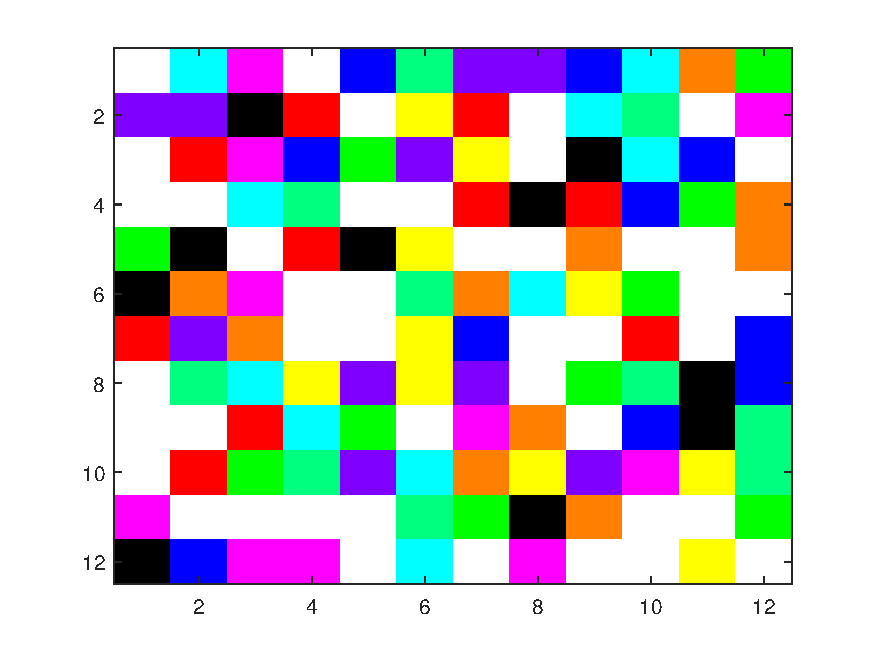
\includegraphics[width=\textwidth]{Voorbeeld12_12_begin}
        \caption{Situation before segregation}
        \label{fig:wis12b}
    \end{subfigure}\hspace{0cm}
    ~ 
    \begin{subfigure}{0.45\textwidth}
        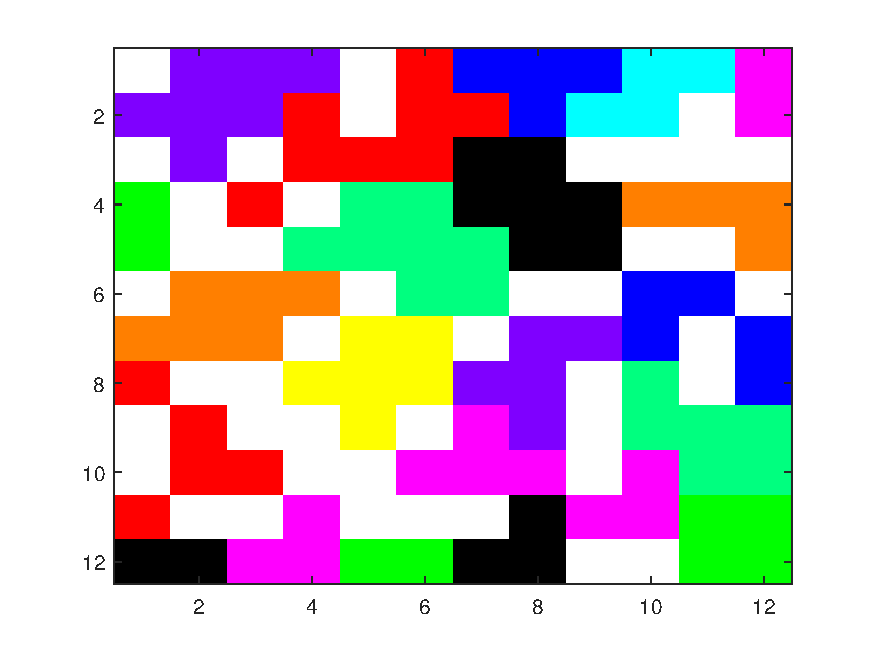
\includegraphics[width=\textwidth]{Voorbeeld12_12_eind}
        \caption{Situation after segregation}
        \label{fig:wis12a}
    \end{subfigure}
    ~ 
    \caption{An illustration of the effect of switching types on the \(12 \times 12\) Board}
    \label{fig:wissel 12}
\end{figure}

A crucial difference between equilibrium with and without switching, is that if switching is allowed, the concentration of the types may differ between the starting board and the equilibrium status. 
This can be seen in figure \ref{fig:wissel 12} as the number of people of the green type decreased from 10 to 8, the yellow type even decreased from 10 to 6. 
As a matter of fact, allowing switching might lead to the extinction of several types. 
This is not generally the case for lower bounds on the happiness rule, but if the happiness rule is increased, several types might cease to exist. Despite this being quite interesting, the extinction of types is not included in this report.\\

\subsection{Average number of generations until equilibrium}

\begin{figure}[H]
	\centering
    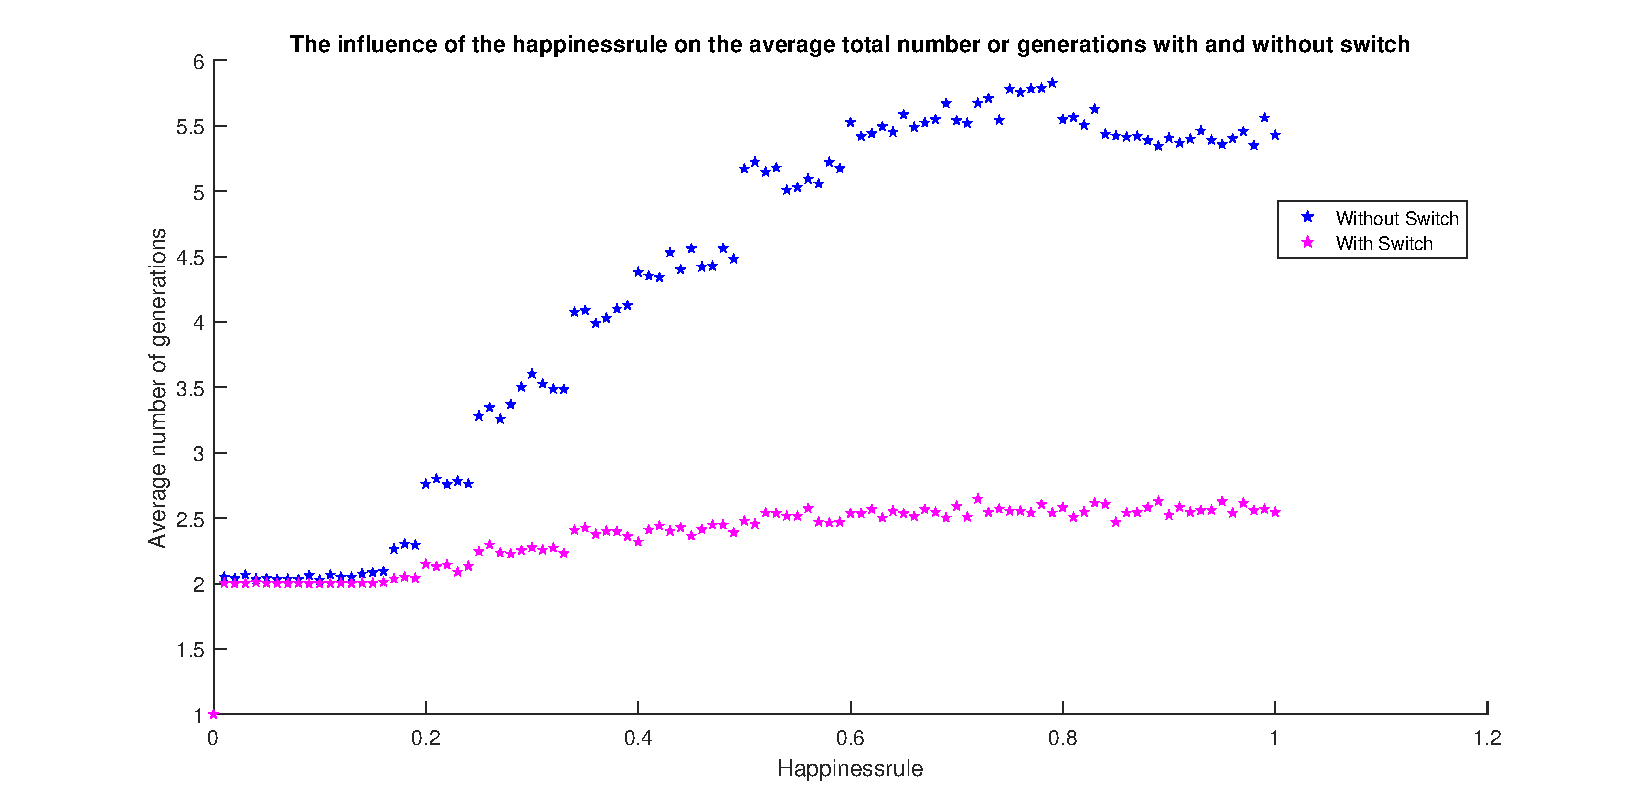
\includegraphics[width=\textwidth]{happinessrule-totaantgenwithswitchorwithoutswitch.pdf}
    \caption{Number of generations until equilibrium on an $8\times 8$ bord with standard setting, with and without type switching}
    \label{fig:AantGenS}
\end{figure}